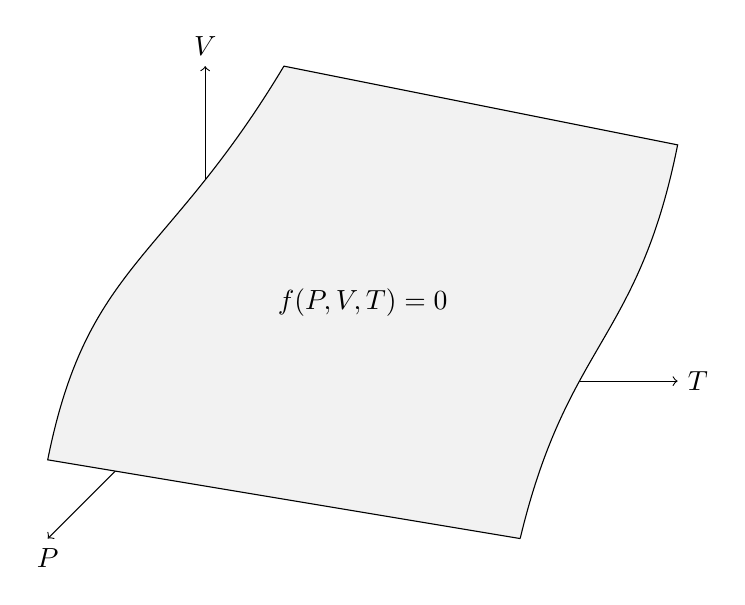
\begin{tikzpicture}[scale=1.0]
  \draw[->] (2,2)--(0,0) node[below=0.2]{$P$};
  \draw[->] (2,2)--(2,6) node[above=0.2]{$V$};  
  \draw[->] (2,2)--(8,2) node[right=0.2]{$T$};
  \draw[fill=gray!10!white] (6,0)--(0,1)..controls(0.5,3.5)and(1.5,3.5)..(3,6)
                                 --(8,5)..controls(7.5,2.5)and(6.6,2.5)..(6,0);
  \draw (4,3) node{$f(P,V,T) = 0$};
\end{tikzpicture}
